\PassOptionsToPackage{top=3cm,left=3cm,right=3cm,bottom=3cm}{geometry}
\documentclass[fleqn,11pt]{wlscirep_supp}

\usepackage[]{minitoc}
\mtcsetdepth{secttoc}{3}
\setcounter{secnumdepth}{2}
\setcounter{tocdepth}{2}
\mtcsettitle{secttoc}{}


\usepackage[utf8]{inputenc}
\usepackage[T1]{fontenc}
\usepackage[english]{babel}
%\usepackage[top=3cm,left=3cm,right=3cm,bottom=3cm]{geometry}% by courtesy of Mico
\usepackage{lmodern}
\usepackage{bbm}
\usepackage{graphicx}
\usepackage{epstopdf}
\usepackage{colortbl}
\usepackage{siunitx}
\sisetup{
  detect-all,
  detect-weight=true,
  detect-family=true,
  mode=text,
%   detect-inline-family=math,
  group-separator={,},
%   group-minimum-digits={3}			
}
\usepackage{rotating}
\usepackage{tabularx}
\usepackage{tabu}
\usepackage{authblk}
\usepackage{mathtools}
\usepackage{overpic}
\usepackage{url}
\usepackage{tikz}
\usetikzlibrary{positioning}
\usetikzlibrary{arrows}
\usetikzlibrary{fit}
\usepackage{multirow}
\usepackage{float}
\usepackage[normalem]{ulem}
\usepackage{bm}
\usepackage{enumerate}
\usepackage[absolute,overlay%,showboxes
                        ]{textpos}
% \usepackage{caption}
\usepackage[font=small,labelfont=bf,justification=justified]{caption}
\usepackage{subcaption}
\usepackage{xspace}
\usepackage[colorinlistoftodos]{todonotes}
\usepackage{placeins}
\usepackage{makecell, booktabs}
\usepackage{eqparbox}
\usepackage{rotating}
\usepackage{graphicx}
\usepackage{xspace}
\usepackage{setspace}
%\usepackage{comment}
\usepackage[resetlabels,labeled]{multibib}
\newcites{Supp}{References}
\usepackage[sort&compress]{cleveref}
\Crefname{appendix}{Supplement}{Supplements}

%\usepackage{mathabx}

% Table formatting packages
\usepackage{dcolumn} % align decimal points in tables
\newcolumntype{d}[1]{D{.}{.}{#1}}
\usepackage{booktabs} 
\usepackage[flushleft]{threeparttable}
\usepackage{siunitx} % align on decimal point in tables
\usepackage{lineno}
\usepackage{etoolbox}

\usepackage{lscape}
\usepackage{longtable}
\usepackage{arydshln}

% math
\usepackage{amsmath,amsfonts,amssymb}
% additional math symbols
\DeclareFontFamily{U}{mathb}{}
\DeclareFontShape{U}{mathb}{m}{n}{
  <-5.5> mathb5
  <5.5-6.5> mathb6
  <6.5-7.5> mathb7
  <7.5-8.5> mathb8
  <8.5-9.5> mathb9
  <9.5-11.5> mathb10
  <11.5-> mathb12
}{}
\DeclareSymbolFont{mathb}{U}{mathb}{m}{n}
\DeclareMathSymbol{\ulsh}{3}{mathb}{"E8}
\DeclareMathSymbol{\ursh}{3}{mathb}{"E9}
\DeclareMathSymbol{\dlsh}{3}{mathb}{"EA}
\DeclareMathSymbol{\drsh}{3}{mathb}{"EB}

%% Patch 'normal' math environments:
\newcommand*\linenomathpatch[1]{%
  \cspreto{#1}{\linenomath}%
  \cspreto{#1*}{\linenomath}%
  \csappto{end#1}{\endlinenomath}%
  \csappto{end#1*}{\endlinenomath}%
}

\linenomathpatch{equation}
\linenomathpatch{gather}
\linenomathpatch{multline}
\linenomathpatch{align}
\linenomathpatch{alignat}
\linenomathpatch{flalign}

\linenumbers

% PLOS formatting
\makeatletter %only needed in preamble
\renewcommand\Large{\@setfontsize\Large{18pt}{18}}
\renewcommand\large{\@setfontsize\large{16pt}{18}}
\makeatother

\addto\captionsenglish{\renewcommand{\figurename}{Fig }}

% \usepackage{xstring}
% \usepackage{etoolbox}
% \usepackage{caption}

% \captionsetup{labelfont=bf,tableposition=top}

% \makeatletter
% \newcommand\formatlabel[1]{%
%     \noexpandarg
%     \IfSubStr{#1}{.}{%
%       \StrBefore{#1}{.}[\firstcaption]%
%       \StrBehind{#1}{.}[\secondcaption]%
%       \textbf{\firstcaption.} \secondcaption}{%
%       #1}%
%       }


% \patchcmd{\@caption}{#3}{\formatlabel{#3}}
% \makeatother

\renewcommand*{\Affilfont}{\normalsize\normalfont}
\renewcommand*{\Authfont}{\normalfont}


% referencing of unnumbered materials and methods
\newcounter{methods}
\renewcommand{\themethods}{Materials and methods}

% Track changes
%\usepackage[markup=underlined]{changes}
\makeatletter
\@namedef{Changes@AuthorColor}{magenta}
\colorlet{Changes@Color}{magenta}
\makeatother


%=====================================================================% Declare

\DeclareSIUnit\eur{\officialeuro}
\DeclareSIUnit\M{M}
\DeclareSIUnit\k{k}

% Widebar symbol
% \DeclareFontFamily{U}{mathx}{\hyphenchar\font45}
% \DeclareFontShape{U}{mathx}{m}{n}{<-> mathx10}{}
% \DeclareSymbolFont{mathx}{U}{mathx}{m}{n}
% \DeclareMathAccent{\widebar}{0}{mathx}{"73}

%=====================================================================% New commands (Macros)

% def
\def\sym#1{\ifmmode^{#1}\else\(^{#1}\)\fi}
\definecolor{darkgreen}{rgb}{0.0, 0.5, 0.0}

% new command
\newcommand{\smallsim}{\smallsym{\mathrel}{\sim}}
\newcommand{\specialcell}[2][c]{%
  \begin{tabular}[#1]{@{}l@{}}#2\end{tabular}}
\newcommand{\specialcellc}[2][c]{%
  \begin{tabular}[#1]{@{}c@{}}#2\end{tabular}}
\newcommand\ie{i.\,e.\xspace}
\newcommand\eg{e.\,g.\xspace}
\newcommand{\dd}[1][]{\mathrm{d}#1}
\newcommand{\BK}[1]{{\color{orange}{BK: #1}}}
\newcommand{\figletter}[1]{{{\fontfamily{\sfdefault}\selectfont \textbf{#1}}}}
\newcommand\TODO[1]{{\color{red}#1}}  
\newcommand{\FIX}[1]{{\color{darkgreen}#1}}  

% renewcommand
\renewcommand\theadfont{\bfseries}
\renewcommand\theadalign{lc}
\renewcommand\cellalign{tl}

\makeatletter

\newbox\@abstract%
\def\abstitle{\textbf{Abstract}}%
\renewenvironment{abstract}{
  \global\setbox\@abstract\vbox\bgroup%
   \noindent
}{%
   \egroup%
}%

\renewcommand*{\Affilfont}{\normalsize\normalfont}
\renewcommand*{\Authfont}{\normalfont}

\addto\captionsenglish{% Replace "english" with the language you use
  \renewcommand{\contentsname}{List of Texts}
}

\def\@maketitle{%
  \newpage
    {\raggedright\fontsize{18pt}{20pt}\selectfont \@title \par}%
    \vskip 0.5em%
    {\large
      \lineskip .5em%
      \begin{tabular}[t]{l}%
        \raggedright \normalsize\mdseries{\@author} %
      \end{tabular}\par}%
      \vskip 1em
%      \raggedright\Large\abstitle\par
%      \vskip 1em
%    {\unvbox\@abstract\par}%
    \par
  \vskip 0.5em
}
  
\makeatother


%\renewcommand{\thesection}{Text \arabic{section}}
\usepackage{titlesec}
\titleformat{\section}{\normalfont\Large\bfseries}{Text \thesection.~#1}{1em}{}
\renewcommand{\thefigure}{\Alph{figure}}
\renewcommand{\thetable}{\Alph{table}}

\begin{document}
\doublespacing
\nolinenumbers

\newcommand{\supp}{SI Appendix}

\title{\LARGE\singlespacing{\textbf{S1 Appendix} \\ \medskip
Transmission of airborne respiratory infections with and without air cleaners in a Swiss school during non-pandemic conditions: A modeling study of epidemiological, environmental, and molecular data}}

% author list
\author[1$\ddag$]{Nicolas Banholzer}
\author[1$\ddag$]{Kathrin Z\"urcher}
\author[2]{Philipp Jent}
\author[3]{Pascal Bittel}
\author[3]{Lavinia Furrer}
\author[1]{Matthias Egger}
\author[4]{Tina Hascher}
\author[1*]{Lukas Fenner}

\affil[1]{Institute of Social and Preventive Medicine, University of Bern, Bern, Switzerland}
\affil[2]{Department of Infectious Diseases, Inselspital, Bern University Hospital, University of Bern, Bern, Switzerland}
\affil[3]{Institute of Infectious Diseases, University of Bern, Bern, Switzerland}
\affil[4]{Institute of Educational Science, University of Bern, Bern, Switzerland}

\affil[*]{Corresponding author: lukas.fenner@ispm.unibe.ch }

\affil[$\ddag$]{These authors contributed equally to this work.}

%\begin{abstract}\normalfont
%The supplementary material contains (1)~the detailed method, (2)~the simulation-based study, (3)~further descriptives, and (4)~the results from the sensitivity analysis.
%\end{abstract}

\flushbottom
\maketitle
\thispagestyle{empty}

%\newpage

\sloppy
\raggedbottom

\newpage

\appendix

\tableofcontents

\listoffigures

\listoftables

%\listoffigures
%\listoftables

\newpage

\section{Epidemiological line list data}\label{sec:case-data}

Table~\ref{tab:epi-data-line-list} shows the line list data for respiratory cases based on epidemiological data.

{\footnotesize\begin{longtable}{l l l l}
    \caption[Line list of respiratory cases over the study period]{Line list of respiratory cases over the study period.}\label{tab:epi-data-line-list} \\
    \toprule
    Class & Date of absence & Date of symptom onset & Date of return \\
    \midrule
    \input ../../results/epi-data/line-list-data
    \bottomrule
\end{longtable}}

{\footnotesize\begin{longtable}{l l l l l}
    \caption[Line list of molecular test results over the study period]{Line list of respiratory cases over the study period.}\label{tab:mol-data-line-list} \\
    \toprule
    Class & Date of test & Weekday & Test result & Pathogen \\
    \midrule
    \input ../../results/mol-data/line-list-data
    \bottomrule
\end{longtable}}

\clearpage

\section{Molecular line list data}\label{sec:mol-data}

Table~\ref{tab:mol-data-line-list} shows the line list data for the laboratory test results from human saliva samples.

\clearpage

\section{Modeling relative risk of respiratory infections}\label{sec:transmission-model}

\subsection{Overall approach}

The aim is to estimate transmission of SARS-CoV-2 and the effects of infection control measures (mask mandates and air cleaners) on the number of new infections with COVID-19. To estimate transmission, our model links two unobserved quantities (the number of new infections and susceptible students) with one observed quantity (the number of new cases among students). Specifically, we link the number of new cases to the number of new infections in the previous days. We then formulate the daily proportion of susceptible students getting infected as a function of the interventions in place. The effects of interventions are estimated with a Bayesian approach, which requires the specification of prior distributions for all model parameters.

\subsection{Notation}

\begin{tabular}{ll} 
$j$  & class \\
$t$ & days since start of study period \\
$Y_{j}$  & total number of students in class $j$ (unobserved)  \\
$N_{jt}$  & number of  new cases among students in class $j$ at day $t$ (observed) \\
$I_{jt}$  & number of new infections in class $j$ at day $t$ (unobserved)  \\
$S_{jt}$  & number of susceptibles in class $j$ at day $t$ (unobserved)  \\
\end{tabular}  


\subsection{Relating the number of new infections to the number of susceptibles and the presence of interventions}

A proportion of the susceptible students $P_{jt}$ gets infected in class $j = 1,\dots,J$ at each day $t = 1,\dots,T$
\begin{align}
    I_{jt} = S_{jt} P_{jt} ~.
\end{align}
This proportion (or probability) can be estimated using a logit link function
\begin{align}
    \Phi_{jt} &= \log\left(\frac{P_{jt}}{1-P_{jt}}\right) \\
    \textrm{logit}^{-1}(\Phi_{jt}) &= \frac{\exp{(\Phi_{jt})}}{1 + \exp{(\Phi_{jt})}} = P_{jt} ~.
\end{align}

In the absence of interventions, the probability of getting infected is constant, \ie $\Phi_{jt} = \beta_j$. It can only change at times when interventions are in place. Let $\theta_{j}^M$ be the effect of mask mandates and let $\theta_{j}^A$ be the effect of air cleaners in class $j$, then
\begin{align}
    \Phi_{jt} = \beta_j + \theta_{j}^M\,{M}_{jt}
    + \theta_{j}^A\,{A}_{jt},
\end{align}
where ${M}_{jt}$ and ${A}_{jt}$ are binary variables indicating whether mask mandates and air cleaners are in place in class $j$ at day $t$.

\subsection{Relating the number susceptibles to the number of infections}

The daily number of susceptibles $S_{jt}$ are computed as the difference between the total number of students $Y_j$ and the cumulative number of infections $C_{jt}$ in the previous days
\begin{align}
    S_{jt} = Y_j - C_{jt} = Y_j - \sum_{s < t} I_{js}~.
\end{align}
We assume that all students are susceptible at the beginning of the study period, despite the fact that some students were vaccinated or already infected with COVID-19 prior to the beginning of our study. Note that varying susceptibility before study onset can be subsumed in the class-specific transmission rate without interventions $\beta_j$.

\subsection{Relating the number new observed cases to the number of new infections}

The expected number $\mu$ of new cases $N_{jt}$ in country $j$ at day $t$ can be derived from the number of new infections in the previous days as 
\begin{equation}
\mu^{N_{jt}} = \sum_{s < t} I_{js} \cdot p_\text{IN}(t-s) ~, 
\end{equation}
where $p_\text{IN}(t)$ denotes the probability distribution of the incubation period, \ie the probability that a new infected subject reports symptoms at day $t$ after the infection. This distribution is estimated from our data as part of fitting the overall model using an informative prior (Section~\ref{subsec:prior-incubation-period}).

The observed number of new cases are modeled to follow a negative binomial distribution, \ie 
\begin{equation}
N_{jt}  \sim  \textrm{NegBinom}\left(\mu^{N_{jt}}, \sigma^{N_{jt}}\right) \label{eq:N} 
\end{equation}
with mean $\mu^{N_{jt}}$, standard deviation $\sigma^{N_{jt}} = \sqrt{\mu^{N_{jt}} \, \left(1 + \frac{\mu^{N_{jt}}}{\phi^N}\right)}$, and an overdispersion parameter $\phi^N$. 


\subsection{Taking into account transmission outside school days}\label{subsec:consider-weekends}

Absences were reported on school days but symptom onset could have occurred on the weekend, \eg a student absent on Monday due to COVID-19 may report Saturday as the day of symptom onset. Some cases may still have gone unreported because the date of absence was the same as the date of symptom onset for the majority of cases (see Fig.~\ref{fig:delay-weights}). Therefore, we distinguish between the transmission rate during and outside schools days, \ie 
\begin{align}
    \beta_j = \alpha_j + \omega, 
\end{align}
where $\alpha_j$ and $\alpha_j + \omega$ are the logit of the probability of getting infected without interventions during and outside school days, respectively. We estimate $\alpha_j$ and $\omega$ from data using informative priors (Section~\ref{subsec:prior-alpha}). We further assume that transmission outside school days is the same regardless of whether they are weekend or vacation days, but we do not incorporate vacation days into the model likelihood. That is, during vacation, the modeling of $N_{jt}$ is ignored but $I_{jt}$ and $S_{jt}$ are still computed.  


\subsection{Seeding phase}

A few cases were reported in the first days of the study period, indicating that the corresponding infections could have occurred before the start of the study. Therefore, we seed the number of new infections and cases before the study period by initiating our model 12~days (double the average incubation period) prior to the start of the study. Before this day, we assume there have been no infections and all students are susceptible.


\subsection{Adjusting for absences and community transmission}

The probability of getting infected may be influenced by factors other than interventions. We account for two such factors. First, we adjust our estimates for the daily proportion of students absent from class. We expect this proportion to decrease the probability of getting infected because absent students cannot infect classmates and, if staying home, they are also less likely to get infected themselves (if not already infected). Second, we adjust our estimates for the risk of community transmission, which we proxy with the average of the median effective reproduction number for the canton of Solothurn, Switzerland\cite{Scire2022}. We expect higher community transmission to increase the probability of getting infected. The modeling parameters of these factors are denoted by $\bm{\gamma}$.


\subsection{Choice of priors for the probability of getting infected without interventions}\label{subsec:prior-alpha}

We choose informative priors for the logit of the daily probability of getting infected in the absence of interventions $\beta_j = \alpha_j + \omega$. First, our prior for $\alpha_j$ is derived from the share of susceptibles by the end of the study period $S_{jT} / Y_j$, \ie 
\begin{align}
    S_{jT} / Y_j = (1 - \textrm{logit}^{-1}(\alpha_j))^{T_{\mathrm{school}}},
\end{align}
where $T_{\mathrm{school}}$ is the number of school days (excluding weekends and vacation), and solving for $\alpha_j$
\begin{align}
    \textrm{logit}^{-1}(\alpha_j) = 1 - \exp\left(\frac{\log(S_{jT} / Y_j)}{T_{\mathrm{school}}}\right) ~.
\end{align} 
Note that $S_{jT} / Y_j$ and correspondingly $\textrm{logit}^{-1}(\alpha_j)$ will be different for each of our probabilistically generated datasets. Fig.~\ref{fig:prior-alpha}a shows the daily proportion of susceptibles getting infected based on the distributions for the proportion of suspected cases being actual cases of COVID-19 (see Fig.~\ref{fig:prior-proportion}). The corresponding distribution for $\alpha_j$ is shown in Fig.~\ref{fig:prior-alpha}b. We choose a prior for $\alpha_j \sim \textrm{Student-t}(\nu = 3, \mu = -4.1, \sigma = 1.6)$ with wider tails than the empirical distribution to accommodate the fact that $\alpha_j$ may be smaller or larger depending on the effects of interventions and adjustment variables.

\begin{figure}[!htpb]
    \centering
    \includegraphics{figures/redcap-supp-prior-alpha.pdf}
    \caption[Prior for the probability of getting infected without interventions]{Prior for the probability of getting infected without interventions. \textbf{(a)}~Empirical distribution for the daily proportion of susceptibles getting infected across classes. The dotted blue line indicates the mean. \textbf{(b)}~Empirical distribution for the logit of the daily proportion of susceptibles getting infected. The dotted blue line indicates the empirical mean. The corresponding choice of prior for the probability of getting infected without interventions $\alpha$ is hown in red. }
    \label{fig:prior-alpha}
\end{figure}

Second, we choose a prior for $\omega \sim \textrm{Normal}(\mu = \log\,0.7, \sigma = 0.2)$ that encodes our prior belief that students will have fewer indoor contacts outside school days and thus lower odds of getting infected. In addition, this informative prior also considers potential underreporting of cases on weekends (see Section~\ref{subsec:consider-weekends}).  

\clearpage

\subsection{Choice of priors for the effects of interventions}

We consider that the mandates may not have been equally effective in all classes. Therefore, we model the effects of mask mandates as $\theta_{j}^M = \textrm{Normal}(\theta^M, \tau)$, where $\theta^M \sim \textrm{Student-t}(\nu = 7, \mu = 0, \sigma = 2.5)$ is the average effect across classes and $\tau \sim \textrm{Student-t}^{+}(\nu = 5, \mu = 0, \sigma = 1)$ is the variation in the effect between classes. 

Air cleaners only applied to three classes and were installed towards the end of the study period when most students may have already been infected. Therefore, we do not estimate variation in the effect between classes but only the average effect. In addition, we choose a prior leaning towards smaller effects, \ie $\theta^A \sim \textrm{Student-t}(\nu = 7, \mu = 0, \sigma = 1)$.

\subsection{Choice of priors for the incubation period}\label{subsec:prior-incubation-period} 

We estimate the distribution of the incubation period from our data as part of fitting the overall model. Our prior choices for the parameters of this distribution are informed by a meta-analysis\cite{McAloon2020}, which reported a Lognormal distribution with $\log \mu \sim \textrm{Normal}(1.63, 0.06)$ and $\log \sigma \sim \textrm{Normal}^{\textrm{+}}(0.50, 0.05)$. The prior for $p_\text{IN}$ is shown in Fig.~\ref{fig:prior-pin}. Note that $p_\text{IN}$ is discretized via $p_\text{IN}(s) = \int_0^{0.5} p_\text{IN}(\tau) \;\text{d}\tau$ for $s = 0$ and $p_\text{IN}(s) = \int_{s-0.5}^{s+0.5} p_\text{IN}(\tau) \;\text{d}\tau$ for $s > 0$, where $p_\text{IN}(\tau) \sim \textrm{Lognormal}(\mu, \sigma)$ is the density of the lognormal distribution. 

\begin{figure}[!htpb]
    \centering
    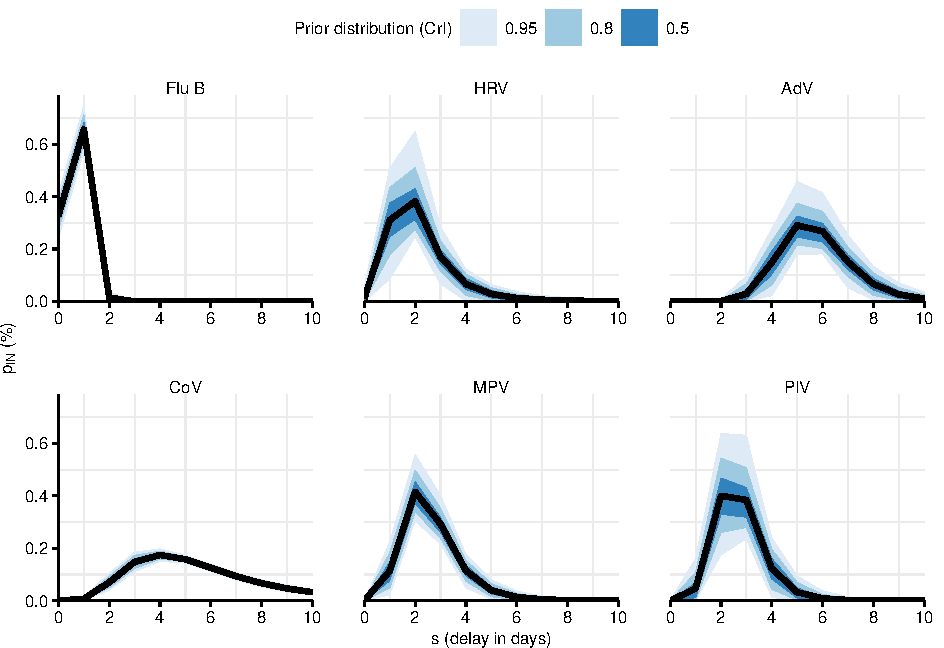
\includegraphics{../../results/epi-data/incubation-periods.pdf}
    \caption[Choices of prior for incubation period]{Choices of prior for incubation period. \textbf{(a)}~Prior for parameter $\log \mu$. \textbf{(a)}~Prior for parameter $\log \sigma$. \textbf{(c)}~Resulting prior $p_\text{IN}$ (posterior mean as line and 50\%, 80\%, and 95\%-quantile as shaded area).}
    \label{fig:prior-pin}
\end{figure}

\subsection{Choice of prior distributions (summary)}

Table~\ref{tbl:prior_choices} provides an overview of the model parameters together with the prior choices. If not tailored to the specifics of the model, our choices are  informed by recommendations on the choice of priors from the Stan Development Team \cite{Stan2020Priors}. 

\begin{table}
\centering
\footnotesize
\begin{tabular}{p{7cm}p{1.5cm}p{6.5cm}}
\toprule
Parameter & Notation & (Hyper-)Prior  \\ 
\midrule
Effects of mask mandates & $\theta_{j}^M$ &  $\textrm{Normal}(\theta^M, \tau)$\\
& $\theta^M$ & $\textrm{Student-t}(\nu = 7, \mu = 0, \sigma = 2.5)$\\
& $\tau$ & $\textrm{Student-t}^{+}(\nu = 5, \mu = 0, \sigma = 1)$ \\
Effects of air cleaners & $\theta^A$ & $\textrm{Student-t}(\nu = 7, \mu = 0, \sigma = 1)$\\
Prob. of getting infected w/o interventions (logit) & $\beta_j$ & $\beta_j = \alpha_j + \omega$ \\
Prob. of getting infected during school (logit) & $\alpha_j$ & $\textrm{Student-t}(\nu = 3, \mu = -4.1, \sigma = 1.6)$ \\
Weekend effect & $\omega$ & $\textrm{Normal}(\mu = \log\,0.7, \sigma = 0.2)$ \\
Overdispersion & $\phi^N$ & $\phi^N = \left(\frac{1}{\xi^N}\right)^2$ \\
 & $\xi^N$ & $\textrm{Normal}^{+}(\mu = 0, \sigma = 1)$ \\
Time from infection to new case & $p_\text{IN}$ & $\textrm{Lognormal}(\log \mu, \log \sigma)$ \\
& $\mu$ & $\textrm{Normal}(\mu = 1.63, \sigma = 0.06)$ \\
& $\sigma$ & $\textrm{Normal}^{\textrm{+}}(\mu = 0.50, \sigma = 0.05)$ \\
Adjustments & $\bm{\gamma}$ & $\textrm{Student-t}(\nu = 7, \mu = 0, \sigma = 2.5)$ \\ 
\bottomrule
\end{tabular}
\caption{Prior choices for model parameters.}
\label{tbl:prior_choices}
\end{table}

\clearpage

\section{Modeling positive rate of human saliva samples}\label{sec:multinomial-model}

\section{Modeling changes in particle concentrations}\label{sec:env-regression-model}

The change in aerosol number concentration $CN_{jt}$ in class $j$ at day $t$ (analogously for particle mass concentrations $PM_{jt}$) is estimated using Bayesian log-linear regression models, \ie
\begin{align}
    \log\,CN_{jt} = \alpha + \beta\,\textrm{School}_j + \bm{\gamma}\,\textrm{Weekday}_t + \theta_M\,M_{jt} + \theta_A\,A_{jt} + \zeta\,\log\,\textrm{N}_{jt} + \omega\,\log\,\textrm{AER}_{jt}~, 
\end{align}
where $\alpha$ is the log of the aerosol concentration without interventions, $\beta$ and $\bm{\gamma}$ are school and weekday effects, respectively, $\theta_M$ and $\theta_A$ are the effects of mask mandates ($M_{jt}$) and air cleaners ($A_{jt}$), respectively, $\zeta$ adjusts for the number of students in class ($\textrm{N}_{jt}$), and $\omega$ adjusts for the outdoor air exchange rate ($\textrm{AER}_{jt}$). The latter is computed from measured indoor CO$_2$ levels (see Section~\ref{sec:rav-computation}). The percent reduction in particle concentrations with interventions are quantified as $100 \times (\mathrm{e}^{-\theta} - 1)\,\%$.

\clearpage

\section{Detailed model results for risk of infection model}\label{sec:detailed-redcap}

Table~\ref{tab:estimation-results} presents the posterior mean, credible intervals and model diagnostics for all model parameters. See the main paper for a discussion of the effects of interventions. Here we briefly discuss some of the additional model parameters.

The effective sample size (ESS) and the Gelman-Rubin convergence diagnostic ($\hat{R}$) indicate good estimation power. It further suggests that the Markov chains converged.

The estimate for $\tau$ indicates that there is variation in the effects of mask mandates between classes. However, the credible intervals of $\theta_j^M$ all include zero, indicating that there is only mild deviation of the class-specific estimates from their cross-class average estimate $\theta^M$.   

The mean estimate for the proportion of students being absent is negative, indicating that higher proportion of absences decrease the probability of getting infected. In contrast to that, the estimate for the reproduction number in the community is positive, indicating that higher community transmission increases the probability of getting infected. Both estimates are in line with our hypothesized effect, although it should be noted that both estimates have large credible intervals including zero.

The overdispersion parameter ($\phi$) cannot be precisely estimated, but the credible intervals indicate rather small overdispersion ($\phi \rightarrow \infty$).

The estimates for the logit of the probability of getting infected during school days without interventions ($\alpha$) are larger than the prior mean. This is due to the reduction in transmission from mask mandates. The weekend effect ($\omega$) is negative, but smaller than the mean of our informative prior, indicating that the likelihood suggests more comparable transmission on weekends.   

The posterior distribution of the parameters of the incubation period ($\mu^{p_{IN}}$ and $\sigma^{p_{IN}}$) are close to their prior, indicating that the data is not informative about the incubation period.  

\begin{table}[!htpb]
    \caption[Estimation results from transmission model]{Estimation results from transmission models across the 100 generated datasets for the number of new cases of COVID-19.}
    \label{tab:estimation-results}
    \footnotesize
    \centering
    \begin{tabular}{lrrrrr}
    \toprule
    Parameter & Mean & Lower 95\%-CrI & Upper 95\%-CrI & $\hat{R}$ & ESS \\
    \midrule
    \input ../../results/epi-data/estimation-results
    \bottomrule
    \multicolumn{6}{p{13cm}}{\scriptsize
        ESS is the effective sample size, \ie the number of independent MCMC samples with estimation power equivalent to the total number of autocorrelated samples\cite{Stan2022}, and $\hat{R}$ is the Gelman-Rubin convergence diagnostic \cite{Gelman1992}. Low ESS or $\hat{R}$ or $\hat{R}>1.10$ indicate bad convergence of the model \cite{Gelman2013}.}
    \end{tabular}
\end{table}

Our model accounts for the delay from infection to case confirmation and allows transmission to change only at the dates of interventions. It thus reflects overall trends in transmission during study conditions rather than day-to-day variation. To evaluate how well our model fits these trends, Fig.~\ref{fig:coverage} compares the estimated number of cases from the probabilistic simulation with the estimated number of new cases from the transmission model. Overall the estimates are in good agreement. The 95\%-CrI of the model-based estimates includes the 95\%-quantile of the simulation-based estimates. 

\begin{figure}[!htpb]
    \centering
    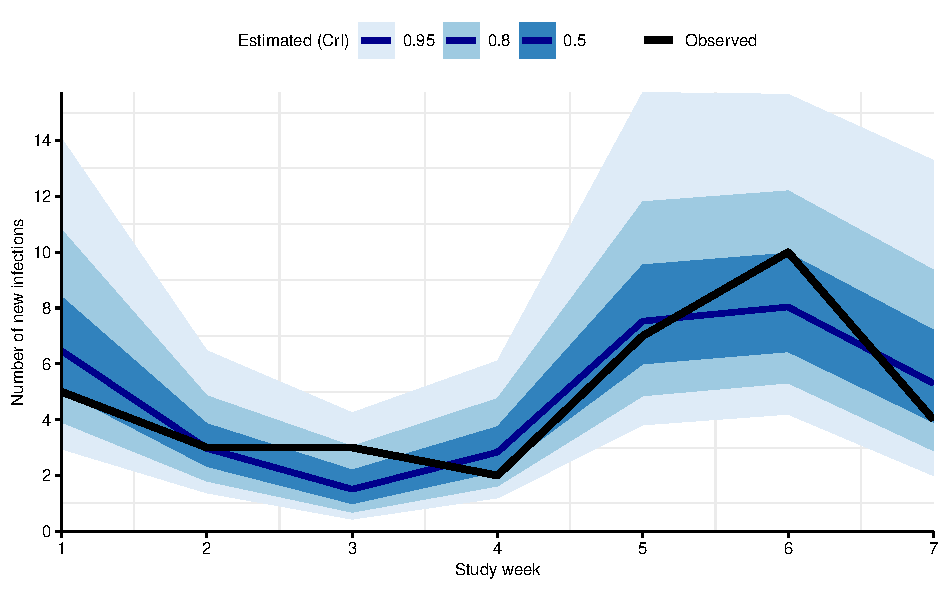
\includegraphics{../../results/epi-data/model-fit.pdf}
    \caption[Model- and simulation-based estimates of the number of COVID-19 cases]{Estimated (posterior mean as dot and 95\%-CrI as line) number of cases from our probabilistic simulation (blue) and transmission model (black).}
    \label{fig:coverage}
\end{figure}

\clearpage

\section{Detailed model results for positivity rate in human saliva samples}\label{sec:detailed-molecular}

\begin{figure}[!htb]
\centering
    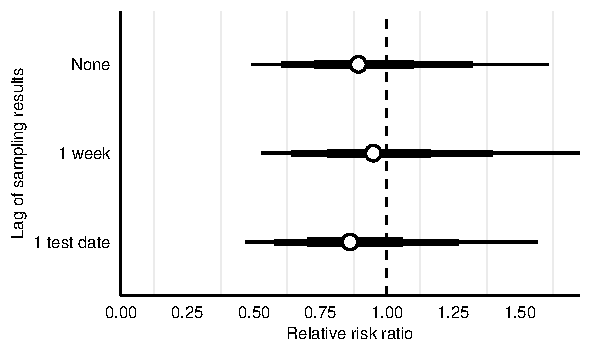
\includegraphics[width=\linewidth]{../../results/mol-data/model-results.pdf}
    \caption[Boxplot of environmental variables by school and study condition]{Boxplot for the daily average values of each environmental variable by school and study condition.}
    \label{fig:mol-estimation-results-sensitivity}
\end{figure}

\clearpage

\section{Detailed model results for changes in particle concentrations}\label{sec:detailed-palas}

In the main paper, we showed results for changes in particle concentrations by study condition and summarized them across schools. In Fig.~\ref{fig:palas-supp-descriptives}, we present additional results disaggregated by schools and including other environmental variables. Furthermore, numerical estimation results for the reduction in particle concentrations with interventions are shown in Table~\ref{tab:palas-est-results}

\begin{figure}[!htb]
\centering
    \includegraphics[width=\linewidth]{../../results/env-data/othVars-boxplot.pdf}
    \caption[Boxplot of environmental variables by school and study condition]{Boxplot for the daily average values of each environmental variable by school and study condition.}
    \label{fig:env-descriptives-other-vars}
\end{figure}

\begin{table}[!htpb]
    \caption[Estimated reduction in aerosol and particle concentrations with interventions]{Estimated reduction in aerosol number (CN) and particle mass (PM) concentrations with interventions (posterior mean and upper and lower estimate from the 95\%-CrI).}
    \label{tab:palas-est-results}
    \centering
    \footnotesize
    \begin{tabular}{l r r r c r r r }
    \toprule
    & \multicolumn{3}{c}{Mask mandate} & & \multicolumn{3}{c}{Air cleaner} \\ \cline{2-4} \cline{6-8}
    Variable & Mean & Lower & Upper & & Mean & Lower & Upper \\
    \midrule
    \input ../../results/env-data/estimation-results-table.tex
    \bottomrule
    \end{tabular}
    
\end{table}

\clearpage

\bibliography{references.bib}

\end{document}